%% -*- coding:sjis -*-
%%
%% 2013-07-20, Koichi Murase, 入力
%%
\begin{question}{第1問}{村瀬}
ハミルトニアンが
\[
  \mathcal{H}=\frac12\sum_{k=1}^2\left(\frac{p_k^2}m + m \omega^2 x_k^2\right)
\]
で与えられる2次元調和振動子の量子力学を考える。ここで$x_k$は座標で$p_k$はその正準運動量、
$m$は質量、$\hbar=h/2\pi$ ($h$はプランク定数)、Uは角振動数である。正準交換関係は
\[
  [x_k,p_l] = i\hbar\delta_{kl},\quad
  [x_k,x_l] = [p_k,p_l] = 0,\quad
  (k,l=1,2)
\]
である。このとき以下の設問に答えよ。
\begin{enumerate}
\item
  生成消滅演算子
  \[
    a_k^\dag = \frac1{\sqrt{2h}}\left(\sqrt{m\omega}x_k - i \frac1{\sqrt{m\omega}} p_k\right),\quad
    a_k      = \frac1{\sqrt{2h}}\left(\sqrt{m\omega}x_k + i \frac1{\sqrt{m\omega}} p_k\right),\quad
    (k=1,2)
  \]
  がみたす交換関係を、$x_k,p_k$の交換関係から導け。また、ハミルトニアン$\mathcal{H}$を生成消滅
  演算子を用いて表せ。
\item\ilabel{Q1.2}
  基底状態$|0\rangle$は、消滅演算子を用いた条件
  \[
    a_k|0\rangle=0,\quad (k=1,2)
  \]
  により定義される。この定義式を、座標$x_k$を変数とする微分方程式に書き換え、対応す
  る基底状態の波動関数$\psi_0(r)$を$r\;(=\sqrt{x_1^2+x_2^2})$の関数として求めよ。ただし、規格化因
  子を定める必要はない。
\item\ilabel{Q1.3}
  ハミルトニアン$\mathcal{H}$の全ての固有状態を基底状態$|0\rangle$と生成演算子で書き表し、それらの
  固有値を求めよ。また、各固有値に対する縮退度を求めよ。
\end{enumerate}
次に2次元の極座標$r,\theta\;(=\tan^{-1}(x_2/x_1))$を用いた解析を行う。以下の設問では簡単のため
$\hbar=m=\omega=1$とおく。必要であれば、2次元のラプラシアンの極座標表示
\[
  \left(\frac{\partial^2}{\partial x_1^2} + \frac{\partial^2}{\partial x_2^2}\right)\psi
  = \frac{\partial^2\psi}{\partial r^2}
  + \frac1r\frac{\partial\psi}{\partial r}
  + \frac1{r^2}\frac{\partial^2\psi}{\partial\theta^2}
\]
を用いてよい。
\begin{enumerate}
\setcounter{enumi}{3}
\item
  波動関数を$\psi=R(r)\Theta(\theta)$と変数分離し、シュレディンガ一方程式に代入する。$\theta$方向の
  方程式を解くと、$R(r)$に関する微分方程式は
  \[
    \frac{d^2R}{dr^2} + \frac1r\frac{dR}{dr}
    + \left(2E-r^2-\frac{n^2}{r^2}\right) R = 0
  \]
  となることを導け。ここで$E$はハミルトニアン$\mathcal{H}$の固有値を表す。また、$n$は角度方向
  の量子数であるが、それがどのような値をとるべきか、理由とともに述べよ。
\item\ilabel{Q1.5}
  設問\iref{Q1.2}で求めた$\psi_0$を用いて$R(r)=f(r)\psi_0(r)$と書き換えると、$f(r)$に対する微分方程
  式は
  \[
    \frac{d^2f}{dr^2} + \frac1r(1-2r^2)\frac{df}{dr}
    +\left(2E-2-\frac{n^2}{r^2}\right)f = 0
  \]
  となる。$f(r)$を
  \[
    f(r) = r^\alpha \sum_{s=0}^\infty f_sr^s,\quad (f_0=1)
  \]
  のようにべき級数展開するとき、$f(r)$が原点$r=0$で発散しないという条件を用いて実
  数パラメータ$\alpha$を決定せよ。
\item
  設問\iref{Q1.5}のペき級数が有限個の項からなるという条件から固有値$E$を求め、設間\iref{Q1.3}で求め
  た固有値(ただし$\hbar=m=\omega=1$とおいたもの)と一致することを示せ。
\end{enumerate}
\end{question}

\begin{question}{第2問}{村瀬}
ある分子$N$個からなる系を考える。それぞれの分子は3つの状態をとる。そのうちの2つの状
態のエネルギーは縮退しており、そのエネルギーの値を0とする。残りの1つの状態のエネル
ギーを$\varepsilon$とする。それぞれの分子は互いに独立とする。この系が温度$T$の熱平衡状態にあると
仮定して以下の設問に答えよ。
\begin{enumerate}
\item
  この系の内部エネルギーを求めよ。
\item
  この系のエントロピーを求めよ。また、$\varepsilon>0,\,\varepsilon=0,\,\varepsilon<0$のそれぞれの場合につ
  いて、$T=0$でのエントロピーを求め、それらの値が異なる理由を説明せよ。
\end{enumerate}
\def\Ne{N_\varepsilon}
エネルギーが$\varepsilon$の状態にある分子の数を$\Ne$とする。以下の設問で必要ならば、二項分布の公式
\[
  (x+y)^N = \sum_{m=0}^N {}_NC_m x^{N-m} y^m
\]
を利用してもよい。
\begin{enumerate}
\setcounter{enumi}{2}
\item 熱平衡状態での$\Ne$の分布関数$P(\Ne)$を求めよ。
\item 熱平衡状態での$\Ne$の平均値$\langle\Ne\rangle$を求めよ。次に、ある温度$T=T_1$において、$\langle\Ne\rangle$が
  $\varepsilon$によってどのように変化するかについて考える。特に、$\varepsilon$が$\pm\infty$に近づく場合の振る舞
  いや$\varepsilon=0$付近の様子に注意して、$\langle\Ne\rangle$を$\varepsilon$の関数として概形を図示せよ。また、温度
  が$T=2T_1$の場合の$\langle\Ne\rangle$の概形も合わせて図示せよ。
\item 熱平衡状態における$\Ne$の分散$\langle\Ne^2\rangle - \langle\Ne\rangle^2$を求めよ。
\item $\langle\Ne\rangle$の$\varepsilon$に対する応答関数
  \[
    \chi = \frac{\partial \langle\Ne\rangle}{\partial \varepsilon}
  \]
  を求めよ。また、$\chi$を$\langle\Ne^2\rangle-\langle\Ne\rangle$を用いて表せ。
\end{enumerate}
\end{question}

\begin{question}{第3問}{村瀬}
以下の設問を通して、自由空間と導波管(金属でできた中空の管)における電磁波の伝搬の違い
について考えよう。
\def\tbE{\tilde{\bm{E}}}
\def\tbB{\tilde{\bm{B}}}
\begin{enumerate}
\item
  電場を$\tbE$、磁場を$\tbB$とすると、真空中のマクスウェル方程式は
  \begin{align*}
    \nabla\cdot\tbE = 0, &\quad \nabla\times\tbE = -\frac{\partial\tbB}{\partial t},\\
    \nabla\cdot\tbB = 0, &\quad \nabla\times\tbB = \frac1{c^2}\frac{\partial\tbE}{\partial t}
  \end{align*}
  と書ける。ここで$c$は真空中の光速度である。これらの式から、次の波動方程式を導け。
  \begin{align*}
    \left(\nabla^2 -\frac1{c^2}\frac{\partial^2}{\partial t^2}\right)\tbE = \bm{0}, \quad &
    \left(\nabla^2 -\frac1{c^2}\frac{\partial^2}{\partial t^2}\right)\tbE = \bm{0}.
  \end{align*}
\end{enumerate}
以下では、$z$方向に伝搬する電磁場の関数形を
\begin{align*}
  \tbE(x,y,z,t) &= \bm{E}(x,y) \exp[i(kz-\omega t)],\\
  \tbB(x,y,z,t) &= \bm{B}(x,y) \exp[i(kz-\omega t)]
\end{align*}
と仮定する(自由空間中を$z$方向に伝搬する電磁波では、電磁場の$z$成分は共にゼロであるが、
境界が存在する場合には、それらは必ずしもゼロではないことに注意せよ)。
\begin{enumerate}
\setcounter{enumi}{1}
\item
  このとき、$k$と$\omega$で表されるある$\gamma$を用いると、$\bm{E}(x,y),\,\bm{B}(x,y)$の$z$成分$E_z,\,B_z$が
  \begin{align}
    \left(\frac{\partial^2}{\partial x^2} + \frac{\partial^2}{\partial y^2} + \gamma^2\right) E_z&= 0, \ilabel{eq:Q3.1}\\
    \left(\frac{\partial^2}{\partial x^2} + \frac{\partial^2}{\partial y^2} + \gamma^2\right) B_z &= 0 \ilabel{eq:Q3.2}
  \end{align}
  という形の方程式を満たすことを示し、そのときの$\gamma^2$を具体的に書き表せ。
\end{enumerate}
次に、図1のような長方形($a>b$)の断面を持つ導波管内を、$z$方向に伝搬する電磁波を考え
る。導波管の壁面は完全導体でできており、内部は真空とする。ただし、壁面の厚さは無視し
てよいものとする。また、$\bm{n}$を壁面の内側を向く単位法線ベクトルとしたとき、壁面での境界
条件は$\bm{n}\times\tbE=\bm{0},\,\bm{n}\cdot\tbB=0$で与えられる。
\begin{enumerate}
\setcounter{enumi}{2}
\item\ilabel{Q3.3}
  変数分離法を用いて、式\ieqref{eq:Q3.1}を$E_z$について解くことを考える。導波管壁面の境界条件に
  注意すると、整数$m,n$を用いて
  \[
    \gamma^2=\frac{m^2\pi^2}{a^2}+\frac{n^2\pi^2}{b^2}
  \]
  と書けることを示せ。また、この整数の組$(m,n)$に対する解$E_z$を求めよ。ただし、$E_z$
  の最大値を$E$とせよ。
\item\ilabel{Q3.4}
  設問\iref{Q3.3}と同じ整数の組$(m,n)$を用いると、式\ieqref{eq:Q3.2}の解は
  \[
    B_z=B\cos\alpha x\cos\beta y
  \]
  と書ける。ただし、
  \[
    \alpha=\frac{m\pi}{a},\quad \beta=\frac{n\pi}b
  \]
  である。このとき、残りの成分$E_x,\,E_y,\,B_x,\,B_y$を求めよ。
\item\ilabel{Q3.5}
  設問\iref{Q3.3}と\iref{Q3.4}で得られた解$\bm{E}(x,),\,\bm{B}(x,y)$のうち、$E_z=0$を満たす特別な場合を考える。
  4つの盤数の組$(m,n)=(0,0),\,(1,0),\,(0,1),\,(1,1)$に対応する電磁場の解のうち、$z$方向
  に伝搬する電磁波を表し、かつ、その振動数が最小となるものはどれか。その最小振動
  数と$(m,n)$を答え、理由も述べよ。
\item
  設問\iref{Q3.5}で$E_z=0$の代わりに、$B_z=0$を満たす場合はどうなるか。同じく、最小振動数
  と$(m,n)$を、理由をつけて答えよ。
\end{enumerate}
\begin{center}
  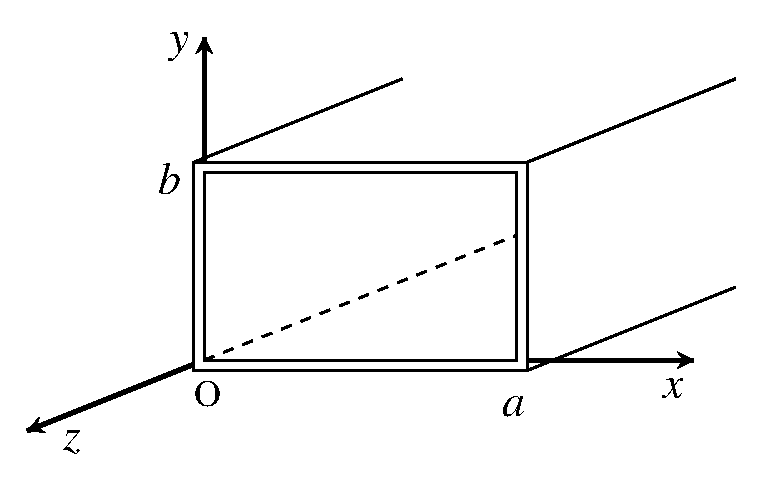
\includegraphics[width=0.56\textwidth]{2007physQ3_1.eps}\\
  図1: $z$方向に無限に伸びている導波管の模式図。ただし、$z<0$ の領域のみ描かれている。
\end{center}
\end{question}

\begin{question}{第4問}{村瀬}
\def\Eg{E_\gamma}
コンプトン散乱を利用して、ガンマ線が飛んでくる方向を測定しよう。光速度を$c$とする。
\begin{enumerate}
\item
  図1のように、エネルギー$\Eg$のガンマ線が静止している電子と衝突し、入射方向から
  角度$\theta$の方向に散乱した。散乱後のガンマ線のエネルギーを$E'_\gamma$、電子の運動量の大きさ
  を$p$、散乱角を$\phi$、電子の静止質量を$m$とする。相対論を考慮して、散乱前後でのエネ
  ルギー保存則と運動量保存則を表す式を書き下せ。
\item
  散乱後のガンマ線のエネルギーは、
  \begin{align}
    E'_\gamma = \frac{\Eg}{1+\alpha(1-\cos\theta)}
  \end{align}
  と与えられることを示せ。ここで$\alpha=\Eg/mc^2$である。
\end{enumerate}
ガンマ線が飛んでくる方向$\theta$を決定するために、ガンマ線検出器A, Bを図2のように$x$軸上
に配置した。これらの検出器はともにNaI(Tl)結晶と光電子増倍管から構成されている。
\begin{enumerate}
\setcounter{enumi}{2}
\item
  この結晶内の原子とガンマ線との相互作用に関して、コンプトン散乱の他に主要な過程
  が2つある。その2つは各々どのような過程か。あわせて150字以内で説明せよ。
\end{enumerate}
ガンマ線が結晶内の原子と相互作用すると電子が散乱される。ここでは、散乱される前の電子
は静止していたものとし、散乱された電子は、結晶内でその運動エネルギーの全てを失うとす
る。したがって、検出器で測定されるエネルギーは、この運動エネルギーであるとしてよい。
図2のガンマ線源Sからは、$\Eg$の単色のエネルギーをもつガンマ線のみが放出される。$\Eg$の
値は既知で、以下では$\Eg<2mc^2$とする。
まず、検出器Aだけでエネルギーの測定を行ったら、図3の度数分布となった。ただし、検出
器のエネルギー分解能は十分高く、また結晶内での多重散乱は無視できるものとする。
\begin{enumerate}
\setcounter{enumi}{3}
\item
  図3の広い分布(I)と鋭いピーク(II)は、ガンマ線と原子との相互作用に関するどのよう
  な過程に対応するか、それぞれ答えよ。また、$E_\mathrm{max}$を$\Eg$と$\alpha$を用いて表せ。
\end{enumerate}
次に、ガンマ線が検出器Aに入射し、結晶内で1回だけコンプトン散乱した後、検出器Bに入
射する事象を考えよう。ここで、検出器A, Bで測定されたエネルギーを、それぞれ$E_\mathrm{A}, E_\mathrm{B}$
とする。
\begin{enumerate}
\setcounter{enumi}{4}
\item
  この場合に得られた$E_\mathrm{A}$と$E_\mathrm{B}$の関係を太線や黒丸で示す図として最も適当なものを図4
  の(あ)$\sim$(か)から1つだけ選び、その理由を簡単に述べよ。ただし、結晶の大きさは
  十分小さいとしてよい。
\item
  検出器Aのエネルギー分解能を考慮して、図2の角度$\theta$の決定精度を考える。まず、角
  度$\theta$を$\Eg,\, E_\mathrm{A},\, \alpha$を用いて表せ。次に、検出器Aのエネルギー分解能を$\Delta E_\mathrm{A}$としたと
  き、角度$\theta$の分解能$\Delta\theta$を、$\Delta E_\mathrm{A},\,E_\mathrm{A},\,\theta,\,\alpha$を用いて表せ。また、$\Eg=mc^2,\,\theta=45$
  度、$\Delta E_\mathrm{A}/E_\mathrm{A}=0.1$のとき、$\Delta\theta$は何度か。有効数字1桁で求めよ。
\end{enumerate}
\begin{center}
  \begin{minipage}{0.45\textwidth}
    \begin{center}
      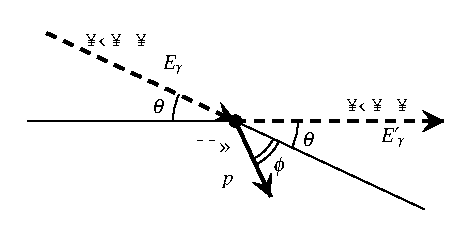
\includegraphics[width=0.8\textwidth]{2007physQ4_1.eps}\\図1
    \end{center}
  \end{minipage}
  \begin{minipage}{0.45\textwidth}
    \begin{center}
      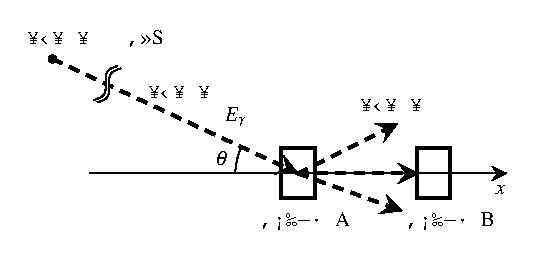
\includegraphics[width=0.8\textwidth]{2007physQ4_2.eps}\\図2
    \end{center}
  \end{minipage}
\end{center}
\begin{center}
  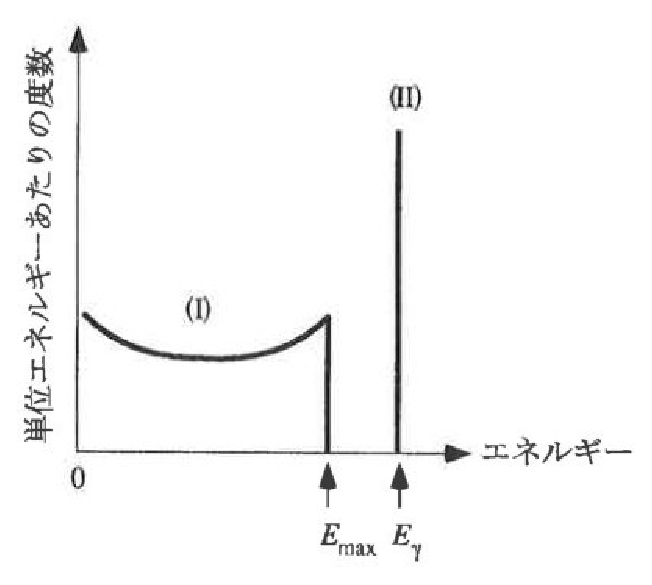
\includegraphics[width=0.4\textwidth]{2007physQ4_3r.eps}\\図3
\end{center}
\begin{center}
  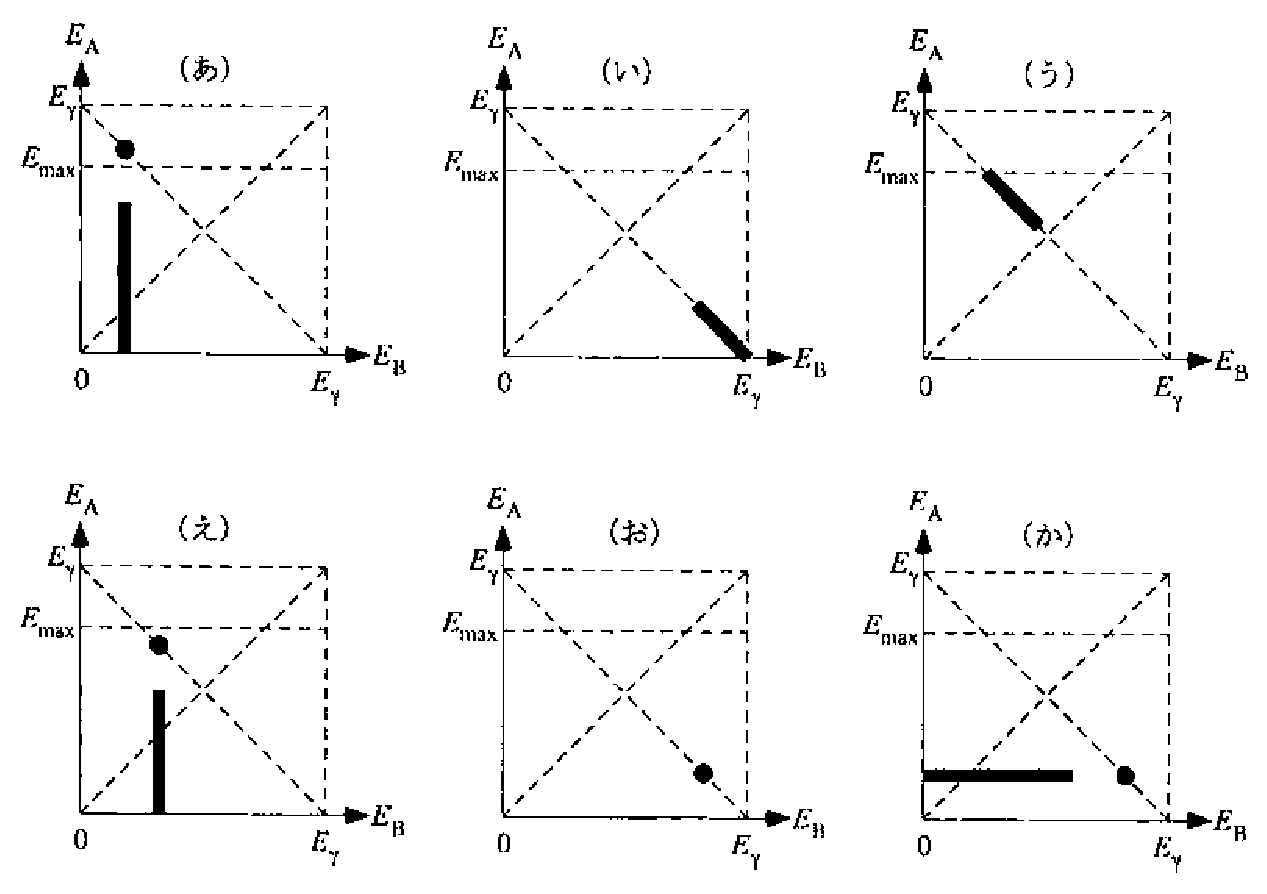
\includegraphics[width=0.8\textwidth]{2007physQ4_4r.eps}\\図4
\end{center}
\end{question}

\begin{question}{第5問}{村瀬}
質量$m$の分子からなる温度$T$の理想気体を考える。その気体中の分子の速度$(v_x,v_y,v_z)$は、
以下のマクスウェル・ボルツマン分布に従っている。
\begin{align}
  f(v_x,v_y,v_z) dv_x dv_y dv_z
  = \left(\frac{m}{2\pi\kB T}\right)^{3/2}
    \exp\left[-\frac{m}{2\kB T}(v_x^2+v_y^2+v_z^2)\right]
    dv_x dv_y dv_z. \ilabel{eq:Q5.1}
\end{align}
ここで、$\kB$はボルツマン定数である。

この速度分布を測定する実験の概略を図1に示す。真空中に、分子源、遮へい板、および直径
$d$の円筒状の回転ドラムが設置されている。それらには、それぞれ小孔A、B、およびHが空
いている(これらはすべてこの紙面上にあるものとする)。分子源内は温度$T$で分子数密度$n$の
単一種類の気体で満ちており、小孔Aから分子が常に一定量噴き出しているとする。ただし、
噴き出すことによって温度や分子数密度は変化しないとする。このドラムは紙面に垂直な中心
軸回りに角速度$\omega$で回転している。ここで、AとBを結ぶ方向を$z$軸とし、$z$軸とドラムの回
転軸が交わる点を$O$とする。

図1(a)のように、Hが$z$軸を通過した瞬間に、分子源から飛んできた分子がドラムの中に入
る。ドラムが回転しているので、図1(b)に示すように、Hが$z$軸からずれてしまうともはや
分子は入れない。ドラムの内側にはフィルムが貼られており、小孔Hから入ってきた分子は、
その速度の遠いに応じてフィルム上の異なる位置に付着し、フィルムを黒化させる。したがっ
て、フィルムの黒化度分布から分子の速度分布を測定することができる。

実験後、フィルムを取り出して黒化度分布$I(s)$を測定すると図2のようになった。ここで、
フィルム上の原点Cを、H-O-Cが一直線になる位置にとり、Cから円周に沿って測ったフィル
ム上での距離を$s$とする。

以下の設問で、必要ならば下記の定積分を用いてよい。
\[
  \int_0^\infty e^{-x^2} dx = \frac{\sqrt{\pi}}2.
\]
\begin{enumerate}
\item
  気体の圧力は、多数の気体分子が壁と衝突してはねかえるときの力積から生じる。その
  衝突を完全弾性衝突と仮定し、式\ieqref{eq:Q5.1}を利用して分子源内の気体の圧力を求めよ。計算過
  程も記述すること。
\item
  式\ieqref{eq:Q5.1}を用いて、分子源の内壁に単位時間、単位面積あたりに衝突する分子数を計算し、小
  孔Aから単位時間あたりに噴き出す分子数を求めよ。ここで小孔Aの面積を$S_\mathrm{A}$とする。
\item\ilabel{Q5.3}
  $z$軸方向に速さ$v$で飛んできた分子がフィルム上に到着する位置$s$を求めよ。また、速さ
  が$v+\Delta v$の分子が到着する位置を$s+\Delta s$としたとき、$\Delta v$と$\Delta s$との関係を求めよ。た
  だし、$\Delta v$は$v$に比べて十分小さいものとする。
\item\ilabel{Q5.4}
  小孔Aから噴き出す分子のうちフィルムに到達するのは、図1(a)に示すように$z$軸まわ
  りの微小立体角$\Delta\Omega$の範囲に噴き出した分子のみである。これを利用して、式\ieqref{eq:Q5.1}を極座
  標表示することにより、ドラムに入る分子のうち、速さが$v$である分子数$N(v)$の$v$依
  存性を求めよ。
\item
  フィルムの黒化度は付着した分子数に比例する。設問\iref{Q5.3}と\iref{Q5.4}の結果から、フィルムの黒
  化度分布叫$I(s)$を求めよ。ただし、$I(s)$の絶対値は$\Delta\Omega$や測定時間(露出時間)などに依
  存するので、$I(s)$の$s$依存性を表す関数形だけを答えればよい。
\item
  上述の実験において、今度は分子源の中に分子量の異なる2種類の気体を入れた場合を
  考える。分子源の温度を一定値$T$に保ったまま測定を行ったときに得られるフィルムの
  黒化度分布$I(s)$の概形を描け。ただし、2種類の気体の混合比は問わないものとする。ま
  た、その結果から、2種類の気体分子の分子量比を求めるにはどうしたらよいか簡単に述
  べよ。
\end{enumerate}
\begin{center}
  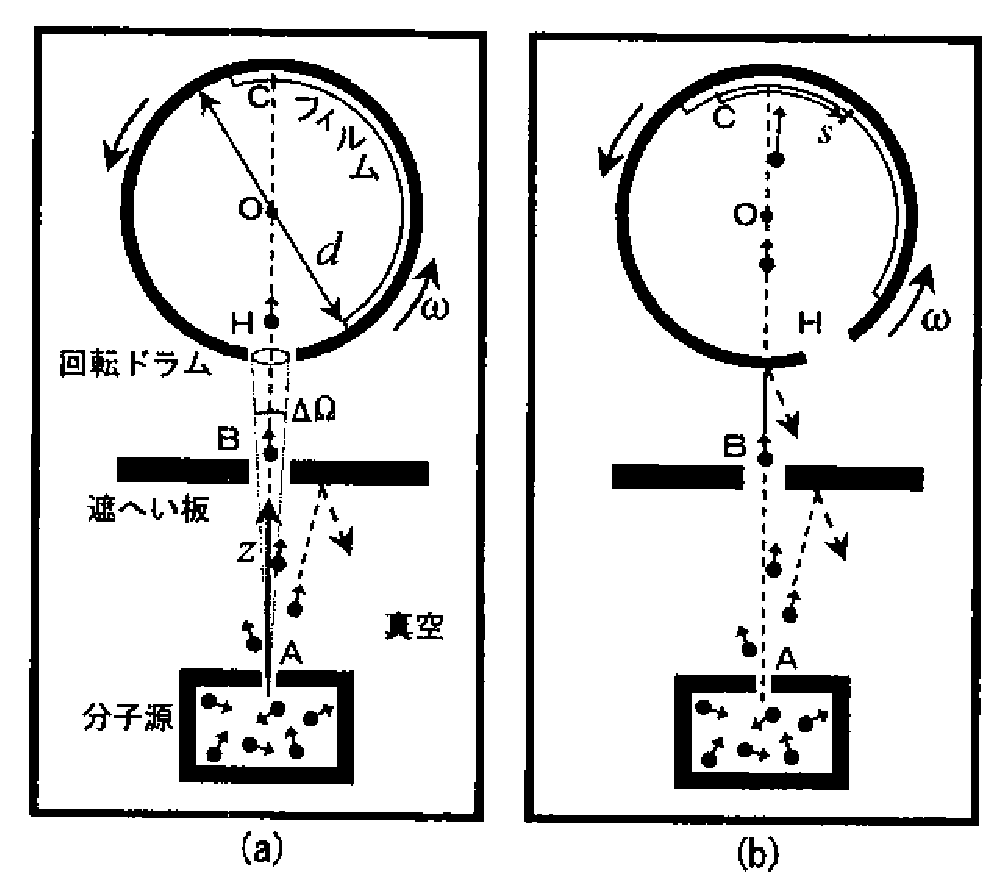
\includegraphics[width=0.6\textwidth]{2007physQ5_1r.eps}\\図1: 分子の速度分布を測定する実験の概略図。
\end{center}
\begin{center}
  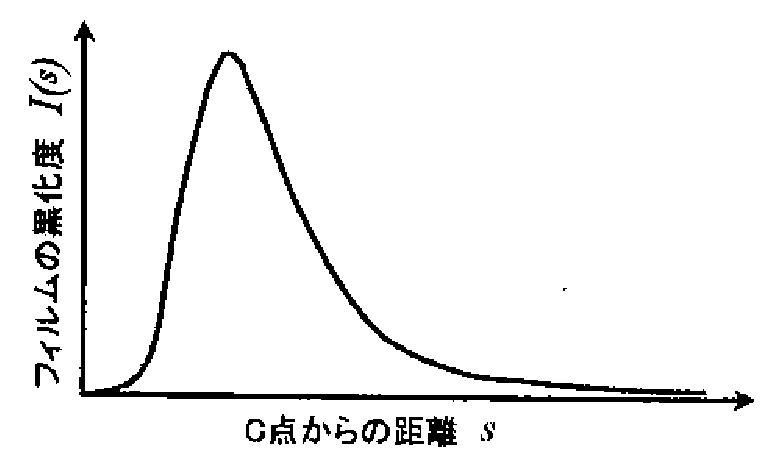
\includegraphics[width=0.5\textwidth]{2007physQ5_2r.eps}\\図2: 実験結果。
\end{center}
\end{question}

\begin{question}{第6問}{村瀬}
基礎的な物理法則を用いて観測量を解釈することで、遠方にある天体の物理量(温度、半径、
密度など)を推定できる。ここでは、黒体放射の性質と古典力学を用いて考察する。

まず、温度$T$の天体からの黒体放射を考える。黒体放射の輝度スペクトル$I_T(\nu)$(単位面積、
単位時間、単位立体角、単位振動数あたりのエネルギー)は、プランクの法則
\begin{align}
  I_T(\nu) = \frac{2h\nu^3}{c^2}\frac1{\exp(h\nu/\kB T)-1} \ilabel{eq:Q6.1}
\end{align}
で与えられる。
ここで、$\nu$は電磁波の振動数、$h$はプランク定数、$c$は光速度、$\kB$はボルツマ
ン定数である。
\begin{enumerate}
\item\ilabel{Q6.1}
  $h\nu/\kB T\ll1$の極限において、$I_T(\nu)$が$\nu,\,T$のそれぞれ何乗に比例するか求めよ。
\item\ilabel{Q6.2}
  $I_T(\nu)$は$\nu=\nu_\mathrm{peak}(T)$にピークを持つ。$\nu_\mathrm{peak}(T)$が$T$に比例することを示せ。また、
  $\nu_\mathrm{peak}(r)=a\times\kB T/h$と置くとき、定数$a$が以下の式を満たすことを示せ。
  \begin{align}
    \frac13a=1-\exp(-a) \ilabel{eq:Q6.2}
  \end{align}
\item
  設問\iref{Q6.1}, \iref{Q6.2}の結果を用いて、$I_T(\nu)$の概形を、$T=10^4$[K]と$10^7$[K]の2つの場合について
  描け。$\nu$を横軸、$I_T(\nu)/I_0$を縦軸とする両対数表示を用いること。ここで、$I_0$は、$T=10^4$
  [K]の輝度スペクトルのピーク値とする。式\ieqref{eq:Q6.2}の近似解を$a=3,\kB/h=2\times 10^{10}$[Hz\,K$^{-1}$]
  として、$\nu_\mathrm{peak}$の値をそれぞれ有効数字1桁で求め、図中に記せ。また、これらピー
  ク付近の電磁波は、一般に何と呼ばれるか、以下の6つからそれぞれ1つずつ選べ。
  \begin{center}
  電波、赤外線、可視光、紫外線、X線、ガンマ線
  \end{center}
\item\ilabel{Q6.4}
  温度$T$の黒体の表面から、単位面積、単位時間あたりに放射されるエネルギー総量を
  $F(T)$とする。式\ieqref{eq:Q6.1}を用いて、$F(T)$が$T$の4乗に比例することを示せ。
\end{enumerate}
次に、高速で自転する天体の力学的な安定性を考える。
\begin{enumerate}
\setcounter{enumi}{4}
\item\ilabel{Q6.5}
  一様な質量密度$\rho$をもち半径が$R$の球形の天体が、周期$P$で自転しているとする。こ
  の天体において最も遠心力の強い場所を考え、そこにおかれた質点(質量$m$)に働く重力
  と遠心力を求めよ。この天体が安定に存在するためには、いかなる場所でも遠心力が重
  力を上回らないことが必要であるという条件から、天体の密度$\rho$の下限値を示せ。なお、
  重力定数は$G$とする。
\end{enumerate}
設問\iref{Q6.4}, \iref{Q6.5}の結果を用い、次のような高密度天体を例にとって、半径と密度および質量の下限値
を推定する。計算結果は有効数字1桁で記せ。
\begin{enumerate}
\setcounter{enumi}{5}
\item\ilabel{Q6.6}
  地球から距離$1.5\times10^{19}$[m]の距離にある天体を観測した。この天体の放射の輝度スペ
  クトルは、温度$T=10^7$[K]の黒体放射であり、地球の位置で観測される単位時間、単
  位面積あたりのエネルギー総量は、$f=3\times10^{-10}$[W\,m$^{-2}$]である(大気の吸収等は無視
  する)。この天体を球形だと仮定したとき、その半径$R$を求めよ。ただし、太陽に関する
  以下の数値を用いてよい。
  \begin{quote}
    太陽は地球から$1.5\times10^{11}$[m]の距離にあり、その半径は$7\times10^8$[m]である。
    太陽からの放射は温度6000[K]の黒体放射であり、地球の位置で観測される
    単位時間、単位面積あたりのエネルギー総量は$f_\mathrm{sun}=1.4\times10^3$[W\,m$^{-2}$]で
    ある。
  \end{quote}
\item
  設問\iref{Q6.6}の天体が、周期$P=1\times10^{-3}$[sec]で自転している。この天体の密度$\rho$の下限値
  を求め、水および原子核の典型的密度と、それぞれ何桁異なるか述べよ。重力定数の値
  として$G=7\times10^{-11}$[N\,m$^2$\,kg$^{-2}$]を用いてよい。また、この天体の質量の下限値を、太
  陽質量$M_\odot=2\times10^{30}$[kg]との比で示せ。
\end{enumerate}
\end{question}
